\section{Vision-Language-Action Models}
\label{sec:vla}

Vision-Language-Action (VLA) models combine large pretrained vision-language models with robot action prediction, pursuing general-purpose control that sees, understands, and acts. Since RT-2 established the paradigm in 2023, VLAs have become the dominant architecture for generalist robot control, with every major humanoid platform---Figure's Helix, NVIDIA's GR00T, Google's Gemini, Physical Intelligence's pi0---adopting a VLA-based brain. Table~\ref{tab:vla} compares the major models.

\begin{table*}[t]
\caption{Comparison of Vision-Language-Action Models}
\label{tab:vla}
\centering
\begin{tabular}{@{}L{2.2cm}cL{2.2cm}L{1.8cm}L{3.2cm}c@{}}
\toprule
\textbf{Model} & \textbf{Year} & \textbf{Backbone} & \textbf{Action Dec.} & \textbf{Key Feature} & \textbf{Cit.} \\
\midrule
RT-1~\cite{brohan2023rt1} & 2023 & EfficientNet & Tokenized & 130K ep., 13 robots & 800+ \\
RT-2~\cite{brohan2023rt2} & 2023 & PaLI-X/PaLM-E & Tokenized & Web knowledge transfer & 400+ \\
OpenVLA~\cite{kim2024openvla} & 2024 & 7B VLM & Tokenized & Open-source, beats RT-2-X & 200+ \\
Octo~\cite{octo2024} & 2024 & Transformer & Diffusion & 800K ep., flexible & 150+ \\
pi0~\cite{black2024pi0} & 2024 & PaLiGemma 3B & Flow match. & 7 robots, 68 tasks & 100+ \\
Gemini~\cite{google2025gemini} & 2025 & Gemini 2.0 & Various & Embodied reasoning & 50+ \\
\bottomrule
\end{tabular}
\end{table*}

\begin{figure}[t]
\centering
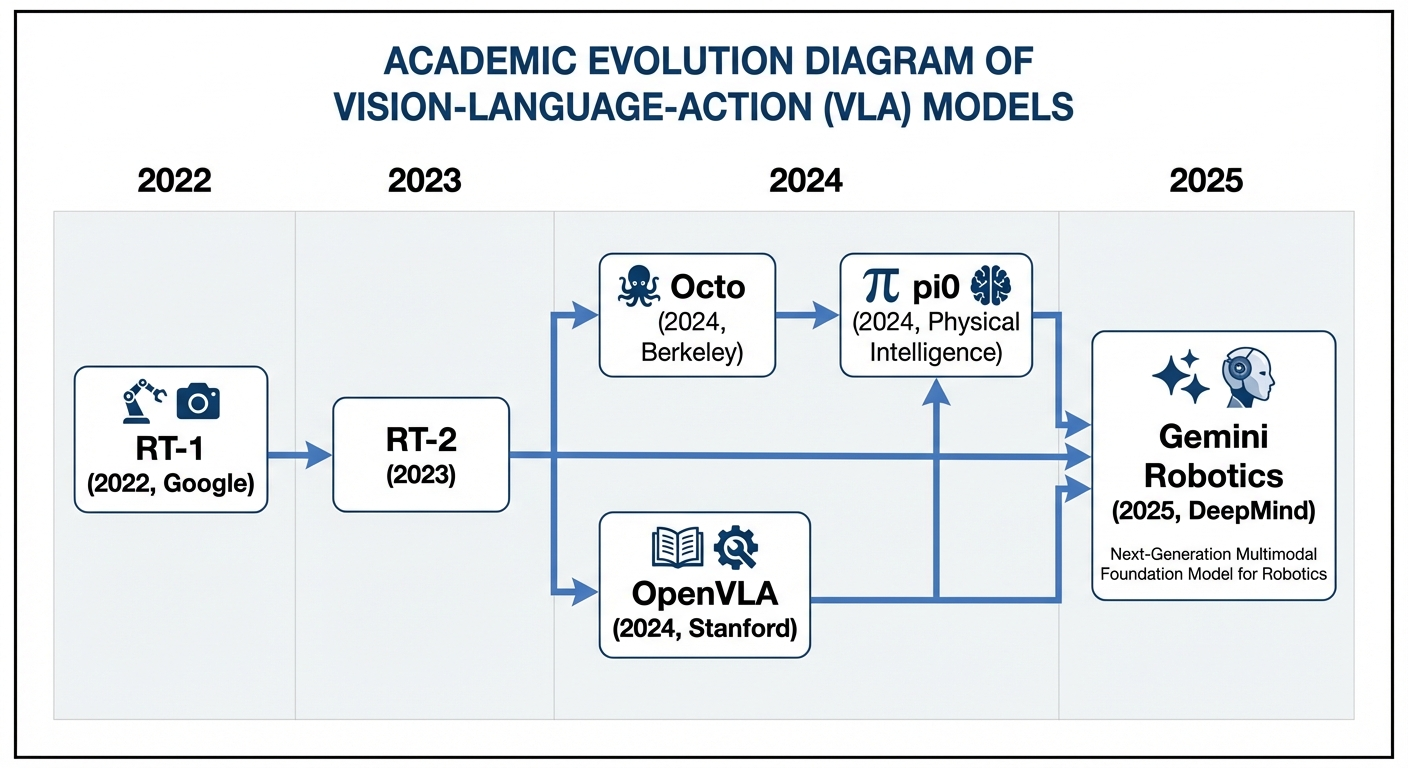
\includegraphics[width=\columnwidth]{../assets/figures/ch08/fig_8_1_vla_timeline_academic.png}
\caption{Evolution of Vision-Language-Action (VLA) models: from RT-1 (2023) through RT-2, OpenVLA, and Octo to pi0 and Gemini Robotics (2025). Each generation expanded the scope of generalist robot control through larger backbones, flow matching decoders, and cross-embodiment training.}
\label{fig:vla_timeline}
\end{figure}

\subsection{The VLA Lineage}

The VLA paradigm has evolved through several inflection points, each expanding the scope of what robot foundation models can achieve:

\textbf{RT-1}~\cite{brohan2023rt1} (Google/Everyday Robots, RSS 2023, 800+ citations) was the first large-scale Transformer trained for real-world robot control, using 130K episodes collected from 13 robots. RT-1 demonstrated that scaling up Transformer architectures and training data yields systematic improvements in manipulation success, establishing the foundation for subsequent models.

\textbf{RT-2}~\cite{brohan2023rt2} (Google DeepMind, CoRL 2023, 400+ citations) \emph{established the VLA paradigm} by fine-tuning large VLMs (PaLI-X with 55B parameters, PaLM-E with 562B parameters) on robot demonstration data. The key insight was that web-scale vision-language knowledge transfers to robotic control: RT-2 could follow novel language instructions involving objects and concepts never seen during robot training, because the underlying VLM had learned these concepts from internet data. This web-to-robot knowledge transfer fundamentally changed the field's approach to generalization.

\textbf{OpenVLA}~\cite{kim2024openvla} (Stanford/Google DeepMind, 2024, 200+ citations) democratized the paradigm with a 7B-parameter model---1/10 the size of RT-2-X---that outperformed RT-2-X while being fully open-source (weights, code, training data). OpenVLA was trained on the Open X-Embodiment dataset and demonstrated that smaller, efficiently trained models can surpass their larger predecessors.

\textbf{Octo}~\cite{octo2024} (UC Berkeley, 2024, 150+ citations) provided a generalist diffusion policy pretrained on 800K episodes from Open X-Embodiment, supporting flexible task and observation definitions with quick fine-tuning---a practical tool for researchers adapting foundation models to new hardware.

\textbf{pi0}~\cite{black2024pi0} (Physical Intelligence, 2024, 100+ citations) introduced a critical innovation: \emph{flow matching}~\cite{lipman2023flow} (ICLR 2023) for action generation. Using a PaLiGemma 3B VLM backbone with a flow matching action expert, pi0 generates actions through continuous normalizing flows rather than iterative diffusion denoising, enabling more efficient action generation. Trained on 7 robots across 68 tasks with 10{,}000+ hours of data, pi0 established the two-stage recipe---large-scale pretraining followed by task-specific post-training---that has become standard.

\textbf{Gemini Robotics}~\cite{google2025gemini} (Google DeepMind, 2025) represents the most ambitious attempt toward a ``universal robot brain,'' building VLA models on the Gemini 2.0 foundation. Gemini Robotics-ER (Embodied Reasoning) adds spatial understanding and grasp prediction to the VLA framework, enabling reasoning about physical interactions before executing them. Its application to dexterous manipulation tasks represents the frontier of VLA capability.

\subsection{Post-Deployment Improvement}

A fundamental limitation of VLA models trained via IL is failure outside the demonstration data distribution. pi0.5/RECAP~\cite{pi2025recap} addresses this through \emph{post-deployment reinforcement learning}: after initial deployment, the system collects success/failure data from real interactions and uses reinforcement learning from execution feedback (RLEF) to continuously improve the policy. This creates a deployment--learning--improvement data flywheel that progressively expands the model's competence boundary without additional human demonstrations---a critical capability for practical deployment where the full range of real-world scenarios cannot be anticipated during initial training.

\subsection{Tactile Integration in VLAs}

Integrating tactile/force information as a first-class modality in VLAs is an emerging but rapidly growing direction. Three approaches have been proposed:

\textbf{ForceVLA}~\cite{yu2025forcevla} (NeurIPS 2025) introduces FVLMoE, a 4-expert Mixture-of-Experts architecture that dynamically routes force, vision, and language inputs based on task demands. Built on a pi0-based VLA backbone, ForceVLA achieves +23.2 percentage points over force-free baselines on contact-rich tasks and maintains 90\% success under visual occlusion---conditions where vision-only models fail catastrophically. The MoE approach partially addresses the temporal resolution mismatch between vision ($\sim$30~Hz) and force/tactile (100--1{,}000~Hz) by enabling task-dependent weighting of modalities.

\textbf{Tactile-VLA}~\cite{huang2025tactilevla} takes a different approach: rather than adding new expert modules, it \emph{unlocks the physical knowledge already present} in the VLA's pretrained vision-language representations. By incorporating a hybrid position-force controller and a reasoning module that adapts strategy based on tactile feedback, Tactile-VLA demonstrates improved generalization on contact-rich tasks without the architectural overhead of MoE.

\textbf{FARM}~\cite{helmut2025farm} (ICRA 2026) integrates high-dimensional GelSight Mini tactile images directly into the Diffusion Policy framework, conditioning action denoising on tactile force profiles to enable force-aware manipulation.

The fundamental challenge remains \textbf{temporal resolution mismatch}: vision operates at $\sim$30~Hz, force/tactile sensors at 100--1{,}000~Hz, and Transformer inference introduces additional latency. No current architecture fully resolves this timing gap, making it one of the top open challenges (Section~\ref{sec:discussion}).

\subsection{Scaling and Data}

VLA performance depends strongly on data scale and diversity. \textbf{Open X-Embodiment}~\cite{oxe2024} (ICRA 2024, 300+ citations) demonstrated this dramatically: the dataset of 1M+ trajectories from 22 embodiments and 34 labs enabled RT-1-X to achieve 50\% improvement and RT-2-X to triple its performance through cross-embodiment training. \textbf{NVIDIA GR00T N1}~\cite{nvidia2025groot} provides the first open humanoid foundation model applying cross-embodiment VLA to manipulation, while GR00T N1.5 added reasoning via Cosmos Reason. NVIDIA's synthetic data pipeline---780K trajectories generated in 11 hours~\cite{nvidia2025synthetic}---demonstrates that simulation can dramatically accelerate the data flywheel when combined with domain randomization.

The systematic analysis ``What Matters in Building VLAs''~\cite{various2025whatmatters} (\emph{Nature Machine Intelligence}, 2025) examined over 600 experimental configurations across 8 VLM backbones and 4 policy architectures, finding that (1)~hierarchical or late fusion architectures outperform early fusion for generalization, and (2)~diffusion decoders consistently outperform tokenized action outputs. These findings align with ForceVLA's MoE architecture (late fusion with dynamic routing) and suggest design principles for future tactile-integrated VLAs.
